% nie rusza�
\RequirePackage{ifpdf}
\newif\ifelektroniczna
\newif\ifjednostronna
\newif\ifprojektInzynierski

%%%%%%%%%%%%%%%%%%%%%%%%%%%%%%%%%%%%%%%%%%%%%%%%%%%%%%%%%%%%%%%%%%%%%%%%%%%%
% USTAWIENIA GLOBALNE I domy�lna �cie�ka do plik�w z obrazkami, kodowanie itp. 
% okre�lone s� w drugiej sekcji ustawie�

% czy projekt czy praca magisterska
%\projektInzynierskitrue % projekt
\projektInzynierskifalse % praca magisterska

% czy wersja elektroniczna (pdf z kolorowymi linkami) czy nie (np. do druku)
\elektronicznatrue
%\elektronicznafalse

% czy jednostronna (recenzent), czy dwustronna (do akt);
% UWAGA: to nie jest dyrektywa dla drukarki; nie zmienia sposobu wydruku, 
% tylko to, w jaki spos�b rozpoczynane s� rozdzia�y, ustawiane marginesy
% itp.

\jednostronnafalse
%\jednostronnatrue

%%%%%%%%%%%%%%%%%%%%%%%%%%%%%%%%%%%%%%%%%%%%%%%%%%%%%%%%%%%%%%%%%%%%%%%%%%%%


% nie rusza�
\ifjednostronna
    \def\strony{oneside,openany}
\else
    \def\strony{twoside,openright}
\fi

\ifpdf
    % uwaga, ustawiaj�c co� innego ni� 12 sprawd� uk�ad strony tytu�owej (marginesy)
    \documentclass[pdftex,12pt,a4paper,\strony,colorlinks,nocenter,noupper,crosshair]{thesis}
    \usepackage[pdftex]{graphicx}
    \pdfcompresslevel=1
\else    
    \documentclass[12pt,a4paper,\strony,nocenter,noupper,crosshair]{thesis}
    \usepackage{graphicx}
\fi

% nie rusza�
\usepackage{url}
\usepackage{stronatytulowa}

%%%%%%%%%%%%%%%%%%%%%%%%%%%%%%%%%%%%%%%%%%%%%%%%%%%%%%%%%%%%%%%%%%%%%%%%%%%%
% USTAWIENIA GLOBALNE - cz�� 2
%

% kodowanie dokumentu
%\usepackage[utf8]{inputenc}   % linuks/windows/mac; pozwala na �atwe mieszanie znak�w z r�nych j�zyk�w
\usepackage[cp1250]{inputenc} % windows

% dane 
\ifprojektInzynierski
    \def\rodzaj{Projekt in�ynierski}
\else
    \def\rodzaj{Praca dyplomowa magisterska}
\fi
%\def\rodzaj{Praca przej�ciowa}

% stan na 2011-2012
\ifprojektInzynierski
    \def\wydzial{Automatyki Elektroniki i~Informatyki}
\else
    \def\wydzial{In�ynierii Biomedycznej}
\fi

\def\tytul{Szacowanie wielko�ci naczynia w badaniach USG} % Prosz� u�y� i ma�ych, i du�ych liter!
\def\autor{Autor: in�. Agata Momot} %Jan Kowalski a NIE JAN KOWALSKI

% tytu� i autor dla pdfa - najcz�ciej jw, ale bez podzia�u na liniie i BEZ POLSKICH LITER
\def\tytulpdf{TYTUL DLA PDFa}
\def\autorpdf{AUTOR DLA PDFa}

% promotor
\def\promotor{Kieruj�cy prac�: dr Jan Juszczyk} % prof. nzw. dr hab. in�. dr n.med doc. Jan Kowalski

% z konsultantem/bez konsultanta
%\def\konsultant{Konsultant: Konsultant} prof. nzw. dr hab. in�. dr n.med doc. Jan Nowak
\def\konsultant{}

\def\data{Gliwice, MIESI�C, ROK} % uwaga na wielko�� liter: grudzie� 2012/czerwiec 2012/..

% do pdfa
\def\slowakluczowe{SLOWA,KLUCZOWE}

% �cie�ka do obrazk�w
\graphicspath{{./rysunki/}}

% ustawienia dla pdfa
\ifpdf
\ifelektroniczna
     \usepackage[pdfusetitle=true,
	  pdfsubject={\tytulpdf},
	        pdfkeywords={\slowakluczowe}, 
		pdfcreator={\autorpdf},
		pdfstartview=FitV,
		linkcolor=blue,
		citecolor=red,
		]{hyperref}
\fi                 
\fi


\usepackage{layout}% poka� marginesy

% Nazwa za��cznik�w 
\def\appendixname{Za��cznik}
%%%%%%%%%%%%%%%%%%%%%%%%%%%%%%%%%%%%%%%%%%%%%%%%%%%%%%%%%%%%%%%%%%%%%%%%%%%%

% nie rusza� (cho� chwilowo niepotrzebne)
%	\author{\autor}
%	\title{\tytul}
%	\date{\data}
%

% === PAKIETY ===

% �adne czcionki dla PDF + ustawienia spolszczaj�ce
\usepackage{t1enc,amsmath}
\usepackage[OT4,plmath]{polski}

% potrzebne dla strony tytu�owej:
\usepackage{helvet} 

% pierwszy paragraf w rozdziale/sekcji powinien by� wci�ty
\usepackage{indentfirst}

% marginesy
%\usepackage{anysize}
%\marginsize{3cm}{2.5cm}{2.5cm}{2.5cm}%LPGD
%\setlength{\textheight}{24cm}
% za spraw� thesis
%\textwidth 150mm
%\textheight 225mm

% czcionki matematyczne
\usepackage{amsfonts}

% rysunki z�o�one z wielu [pod]rysunk�w
\usepackage{subfig}
\captionsetup[subfigure]{justification=centerfirst}

% mo�liwo�� sklejania wierszy tabeli
\usepackage{multirow}

% mo�liwo�� wklejania adres�w - jest ju� w��czony wy�ej
%\usepackage{url}

% ulepszona obs�uga cytowa�
\usepackage{cite}

% listingi
\usepackage{listings}
% domy�lne ustawienia (niestety utf8 nie jest akceptowany)
%\lstset{language={Matlab},inputencoding=cp1250}}
%\lstset{language={Matlab},inputencoding=latin2}}
\lstset{language={Java},inputencoding=latin2} % powinno pasowa� te� do C#

% \addcontentsline nie dzia�a za dobrze w po��czeniu z hyperref, ale to nie dzia�a z klas� thesis
%\usepackage[nottoc]{tocbibind}

% strona po cleardoublepage powinna by� pusta, nie z nag��wkami
\usepackage{cleardpempty}

% == opcjonalne

% wymu� po�o�enie grafiki (itp.) przez [H]
\usepackage{float} 

% znak promila i inne znaki specjalne
%\usepackage{textcomp}

% je�li trzeba obr�ci� stron� (wstawi� co� w orientacji poziomej), u�yj tych pakiet�w
%\ifpdf\usepackage{pdflscape}\else\usepackage{lscape}\fi

% je�li potrzebujesz d�ugich tabeli (wiele stron)
%\usepackage{longtable}

% === POLECENIA DODATKOWE ===

% wektor w tek�cie
\def\vec#1{\ensuremath{\mathbf{#1}}}

% anglicyzmy i �acinizmy
\def\ang#1{ang.~\emph{#1}}
\def\lat#1{�ac.~\emph{#1}}

% proste e (jako podstawa logarytmu naturalnego) we wzorach i w tek�cie:
\def\e{\ensuremath{\textrm{\normalfont{}e}}}

% znak stopnia [jak w "5 stopni"]
\def\stopien{\ensuremath{^{\circ}}\protect\space}

% notatki na marginesie
\def\fixme#1{\marginpar{\tiny{}#1}}
%\def\fixme#1{} % gdy nie chcemy ich drukowa�, wystarczy zast�pi� powy�sze tym

%ODNOSNIKI 
% �eby wykorzysta� przypis dwukrotnie; druga wersja gorzej dzia�a�a w po��czeniu 
% z hyperref; czyli \footnote{blablabla \label{przypisX}} + \footnotereuse{przypisX}
%\newcommand{\footnreuse}[1]{\raisebox{1ex}{\scriptsize{}\protect\ref{#1}}}

% == �RODOWISKA DLA TWIERDZE�, LEMAT�W itp. ===
\newtheorem{twierdzenie}{Twierdzenie}[chapter]
\newtheorem{wlasnosc}{W�asno��}[chapter]
\newtheorem{lemat}{Lemat}[chapter]
\newenvironment{dowod}{\parindent=0pt{\bf Dow�d. }}{\begin{flushright}$\square$\end{flushright}}

% === RACZEJ NIE RUSZA� ===

%\usepackage{makeidx}
%\makeindex
%\usepackage{threeparttable}
%\usepackage[small,center]{caption2}

\def\captionlabeldelim{.}

%\usepackage{geometry}
%GATHER{thesis.bib}
%\usepackage[twoside]{geometry}
%\geometry{ lmargin=3.5cm, rmargin=2.5cm, tmargin=3cm, bmargin=3cm,
%headheight=1cm, headsep=0.5cm, footskip=0pt }

\linespread{1}
\chapterfont{\Huge\bfseries}
\sectionfont{\bfseries\Large}
\subsectionfont{\bfseries\large}
\institutionfont{\bfseries}%\mdseries}
\def\captionlabelfont{\bfseries}

\renewcommand{\figureshortname}{Rys.}
\renewcommand{\tableshortname}{Tab.}

\renewcommand\floatpagefraction{.9}
\renewcommand\topfraction{.9}
\renewcommand\bottomfraction{.9}
\renewcommand\textfraction{.1}
\setcounter{totalnumber}{50}
\setcounter{topnumber}{50}
\setcounter{bottomnumber}{50}

\newcommand{\topcaption}{%                  % robi podpis nad tabelk� z odst�pem po podpisie
   \setlength{\abovecaptionskip}{0pt}%
   \setlength{\belowcaptionskip}{10pt}%
   \caption}



% marginesy
\usepackage{anysize}
\marginsize{3cm}{2.5cm}{2.5cm}{2.5cm}%LPGD
%\setlength{\textheight}{24cm}
% za spraw� thesis
%\textwidth 150mm
%\textheight 225mm

\begin{document}
%
\bibliographystyle{acm}
%

%
\stronatytulowa
\titlepage
\ \cleardoublepage % je�li dwustronnie, to druga strona powinna by� pusta
\frontmatter 
%\maketitle

%\tocbibname

\tableofcontents \listoffigures \listoftables
%\listofacros
%\input{abbrev_body}
%\newpage
%\input{spis_oznaczen}

\mainmatter % <--- to + frontmatter powy�ej odpowiada za fakt, �e numerowanie jest od 1!





\chapter{Wst�p}
Post�p medycyny niew�tpliwie z roku na rok staje si� coraz wi�kszy. Takie dzia�anie motywuje przede wszystkim ch�� poprawy og�lnego zdrowia spo�ecze�stwa, prowadz�c do wyd�u�enia �redniego �ycia ludzi jak i nierzadko zapobiegania przedwczesnej �mierci. Prowadzone s� stale liczne badania maj�ce na celu: szybkie stawianie diagnoz, klasyfikacj� nowo odkrytych chor�b, rozw�j coraz to skuteczniejszych i mniej inwazyjnych metod lecenia czy udoskonalanie metod profilaktyki, w tym wdra�anie szczepie� zapobiegaj�cym nowym jednostkom chorobowym. Istotna jest wi�c wsp�praca pomi�dzy �rodowiskiem medycznym jak i naukowym w celu osi�gania coraz to lepszych rozwi�za�. \\
\indent Opr�cz rozwoju medycyny, wiele obszar�w �ycia ludzkiego stale d��y do polepszenia jego og�lnej jako�ci. Post�p cywilizacyjny niezwykle szybko dostarcza nam nowych rozwi�za� technologicznych. Okazuje si�, �e wsp�dzia�anie z pozoru rozbie�nych dziedzin mo�e przynie�� bardzo dobre rezultaty. Takim przyk�adem mo�e by� medycyna i rozw�j nowych technologii, kt�re znajduj� szerokie zastosowanie w profilaktyce i diagnostyce chor�b (np. aparaty do diagnostyki obrazowej: USG-- ultrasonografia, TK-- tomografia komputerowa, MR-- rezonans magnetyczny), planowaniu i nawigacji chirurgicznej \cite{sakasTrendsMedicalImaging2002} (np. systemy �ledz�ce, okulary do rozszerzonej rzeczywisto�ci VR (ang. \textit{Virtual Reality}), wspomaganiu zabieg�w chirurgicznych i rehabilitacji (np. ramiona robot�w) projektowaniu i wytwarzaniu implant�w (r�wnie� z wykorzystaniem druku 3D) oraz monitorowaniu aktywno�ci fizycznych i prowadzeniu zdrowego stylu �ycia (np. mobilne aplikacje oraz opaski sportowe) \cite{phillipsAdvancesHealthTechnology2019}.\\
\indent Niew�tpliwie ka�dy z przytoczonych przyk�ad�w przynosi wiele korzy�ci. Nale�y jednak podkre�li�, �e wczesna diagnostyka chor�b mo�e mie� najwi�ksze znaczenie w odniesieniu do przywr�cenia zdrowia lub zachowania �ycia. Diagnostyka, nie licz�c dzia�a� profilaktycznych, stanowi pierwszy i nierzadko decyduj�cy krok prowadz�cy do ca�kowitego wyleczenia lub podtrzymania �ycia pacjenta. Diagnoza medyczna, w zale�no�ci od przypadku, mo�e polega� na ocenie pojawiaj�cych si� objaw�w, bada� laboratoryjnych, bada� obrazowych lub po��czeniu kilku procedur. Etap ten jest bardzo wa�ny, bior�c pod uwag� czas potrzebny na okre�lenie jednostki chorobowej oraz zgodno�� postawionej diagnozy z rzeczywisto�ci�. \\
\indent Z biegiem czasu coraz cz�ciej obserwuje si� nowe rozwi�zania wspieraj�ce diagnostyk� obrazow�. Mog� one polega� na segmentacji i/lub oceny danego regionu zainteresowania jako obszar zmieniony (lub nie) chorobowo. Mo�liwa jest r�wnie� dok�adniejsza klasyfikacja pod k�tem ustalenia jednostki chorobowej lub szacowanie i analiza wielko�ci takich jak np. d�ugo��, �rednica czy obj�to�� obserwowanych struktur (np. naczynia krwiono�ne, organy, ko�ci). Czynnikami motywuj�cymi wdra�anie takich system�w jest przede wszystkim wi�ksza wydajno�� i dok�adno�� automatycznych, wspomaganych komputerowo system�w w stosunku do samodzielnej diagnozy, opartej na wiedzy lekarskiej. Co wi�cej, zalet� takich rozwi�za� jest pomini�cie czynnika ludzkiego, kt�ry mo�e doprowadzi� do b��dnych wniosk�w, zagra�aj�cych bezpo�rednio zdrowiu i �yciu pacjenta. Naturalnym jest nie dopuszczenie do pe�nej automatyzacji w kwestii dzia�a� medycznych, jednak wsparcie takich narz�dzi mo�e przynie�� ogrom korzy�ci. Systemy te mog� opiera� si� na klasycznych metodach przetwarzania obrazowego jak i wykorzystaniu sztucznej inteligencji AI (ang. \textit{Artificial Intelligence}). W dalszej cz�ci pracy temat ten zostanie przybli�ony \cite{amishaOverviewArtificialIntelligence2019, chenMachineLearningPrediction2017, shenArtificialIntelligenceUltrasound2021a}. 


\section{Wprowadzenie teoretyczne}
Wprowadzenie do tematyki pracy zosta�o podzielone sekcje dotycz�ce kolejno: zasady dzia�ania, przebiegu badania USG, zastosowania ultrasonografii oraz wykorzystania w przypadku obrazowania naczy� krwiono�nych (\ref{ultr}), kaniulacji �y� obwodowych (\ref{kan}), diagnostyki obrazowej wspomaganej komputerowo (\ref{diag}), z podzia�em na tradycyjne metody i te z wykorzystaniem AI oraz standardu DICOM (\ref{dic}). Na ko�cu zosta�a przybli�ona tematyka okre�lania wielko�ci naczy� krwiono�nych na podstawie obraz�w USG (\ref{wielkosc}).

\subsection{Ultrasonografia}\label{ultr}
Do bada� obrazowych mo�emy zaliczy� przede wszystkim: USG, TK, MR, pozytonow� tomografi� emisyjna PET (ang. \textit{Positron Emission Tomography}) oraz tomografi� emisyjn� pojedynczych foton�w SPECT (ang. \textit{Single-Photon Smission Computed Tomography}). Ka�de z przytoczonych modalno�ci podlega innej charakterystyce. W zale�no�ci sytuacji pacjenta dobiera si� odpowiednie badanie.\\
\indent Termin ultrad�wi�ki (fale akustyczne) odnosi si� do cz�stotliwo�ci, kt�re przekraczaj� 20 kHz. Jest to granica traktowana jako g�rna cz�stotliwo��, jak� mo�e us�ysze� ludzkie ucho. Zazwyczaj systemy ultrad�wi�kowe dzia�aj� w zakresie cz�stotliwo�ci od 2 MHz do 20 MHz. Badanie przeprowadza si� przy u�yciu specjalnej aparatury, kt�ra poprzez g�owic� wysy�a do wn�trza organizmu fale ultrad�wi�kowe. Powstaj� one dzi�ki zawartym w g�owicy piezoelektrykom i odwrotnemu zjawisku piezoelektrycznym. Polega ono na zdolno�ci kryszta��w piezoelektrycznych do odpowiadania na zadany sygna� elektryczny mechaniczn� deformacj� i tym samym wytwarzaniem fali mechanicznej (ultrad�wi�kowej). Te nast�pnie odbijaj� si� od badanych tkanek. Powracaj�ce fale trafiaj� spowrotem do g�owicy, gdzie zachodzi proste zjawisko piezoelektryczne. W wyniki poddania niekt�rych kryszta��w
mechanicznym napr�eniom (�ciskaniu lub rozci�ganiu) generowany zostaje potencja� elektryczny, kt�ry zostaje zmierzony i odpowiednio przetworzony (Rys. \ref{piez}) \cite{mastersthesis, ali2008signal}.\\
\begin{figure} 
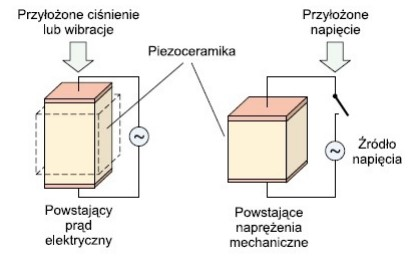
\includegraphics[width=0.8\textwidth]{piezo}
\centering
\caption{Schemat zjawiska piezoelektrycznego \cite{mastersthesis}.}\label{piez}
\end{figure}
\indent Podczas badania USG dochodzi do kilku zjawisk: odbicie, rozproszenie (op�r akustyczny), t�umienie (os�abienie) oraz za�amanie (refrakcja) (Rys. \ref{zjawiska}).
\begin{figure} 
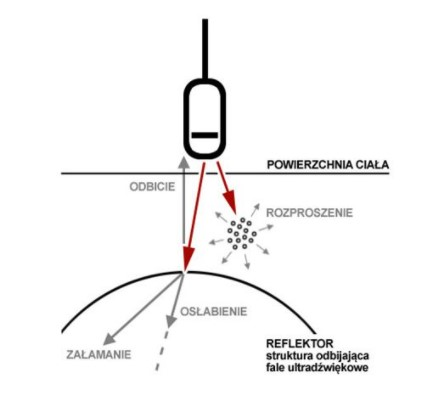
\includegraphics[width=0.7\textwidth]{zjawiska}
\centering
\caption{Zjawiska zachodz�ce po emisji fali USG \cite{SPARQNewWay}.}\label{zjawiska}
\end{figure}
Wykorzystanie zjawiska odbicia fali na granicy o�rodk�w o r�nych g�sto�ciach (r�na pr�dko�� rozchodzenia si� fali) powoduje odbi�r ultrad�wi�k�w w r�nych odst�pach czasu, co pozwala na ocen� wielko�ci, kszta�tu i struktury narz�d�w, a w szczeg�lno�ci r�nicowanie zmian o charakterze litym od zmian o charakterze p�ynowym. Do obrazowania wykorzystywana jest cz�� odbita fali w postaci tzw. powracaj�cego echa, kt�re analizowane jest pod k�tem po�o�enia i intensywno�ci. Po komputerowym przetworzeniu danych, na ekranie widoczne s� punkty odpowiadaj�ce umiejscowieniom odbicia fal. Intensywno�ci echa przyporz�dkowane s� odpowiednim odcieniom ze skali szaro�ci-- od tonu najciemniejszego (kolor czarny) dla braku lub bardzo ma�ej intensywno�ci echa, do koloru bia�ego odpowiadaj�cego du�emu nat�eniu \cite{ali2008signal}.\\

\indent Mo�emy wyr�ni� 3 typy g�owic USG:
\begin{itemize}
\item[�] Liniowa-- zawiera szereg element�w piezoelektrycznych ustawionych wsp�liniowo. Otrzymany obraz jest obszarem prostok�tnym. G�owice liniowe pozwalaj� uzyska� najdok�adniejszy obraz.
\item[�] Sektorowa-- elementy piezoelektryczne s� umieszczone na obrotowym wirniku, co pozwala na zastosowanie mniejszej ich liczby. G�owice sektorowe charakteryzuj� si� znacznie szerszym obszarem wi�zki ni� g�owice liniowe, ale zazwyczaj du�o gorszymi parametrami rozdzielczo�ci. 
\item[�] Konweksowa-- jest rozwi�zaniem po�rednim mi�dzy g�owic� sektorow� a liniow�. Pozwala uzyska� znacznie dok�adniejsze obrazy ni� g�owica sektorowa, a pole obserwacji jest du�o wi�ksze ni� w przypadku g�owicy liniowej \cite{ali2008signal}.
\end{itemize}
\indent Obrazowanie ultrasonograficzne to nieinwazyjna i tania metoda, dostarczaj�ca wynik�w w czasie rzeczywistym w przeciwie�stwie do pozosta�ych metod. Zapewnia wiele korzy�ci takich jak brak promieniowania jonizuj�cego oraz zapewnia ci�g�e obrazowanie wideo w czasie rzeczywistym. Dodatkow� zalet� jest bezbolesno�� badania. Niestety USG posiada r�wnie� kilka wad. Spo�r�d wymienionych bada� ultrasonografia jest jedn� z najmniej dok�adnych metod i podatn� na szumy, objawiaj�ce si� niewyra�nym obrazem \cite{cheUltrasoundRegistrationReview2017a, ali2008signal}. Na rysunku \ref{porownanie} przedstawiono zestawienie przyk�adowych obraz�w poszczeg�lnych metod obrazowania.

\newcounter{wielo}[figure]
\renewcommand\thewielo{\alph{wielo}}
    \def\captionlabeldelim{.}
    \def\figurename{Rysunek}
	\setcounter{wielo}{0}
\begin{figure}[h]
	\centering
	\setlength{\fboxsep}{0pt}
	\begin{minipage}[t][][c]{4cm}
	\centering 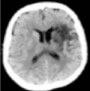
\includegraphics[width=0.85\textwidth]{CT}\\
	(\refstepcounter{wielo}\label{CT}\alph{wielo})
	\end{minipage}%
	\begin{minipage}[t][][c]{4cm}
	\centering 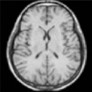
\includegraphics[width=0.85\textwidth]{MR}\\
	(\refstepcounter{wielo}\label{MR}\alph{wielo})
	\end{minipage}
	\begin{minipage}[t][][c]{4cm}
	\centering 
\includegraphics[width=0.85\textwidth]{PET}\\
	(\refstepcounter{wielo}\label{PET}\alph{wielo})
	\end{minipage}
	\begin{minipage}[t][][c]{4cm}
	\centering 
\includegraphics[width=0.85\textwidth]{SPECT}\\
	(\refstepcounter{wielo}\label{SPECT}\alph{wielo})
	\end{minipage}
	\begin{minipage}[t][][c]{4cm}
	\centering 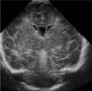
\includegraphics[width=0.85\textwidth]{USG}\\
	(\refstepcounter{wielo}\label{USG}\alph{wielo})
	\end{minipage}
    \captionsetup{justification=centering}
	\caption{Por�wnanie obrazowania m�zgu za pomoc� r�nych metod: TK (\ref{CT}), MR (\ref{MR}), PET (\ref{PET}), SPECT (\ref{SPECT}), USG (\ref{USG}) \cite{el-gamalCurrentTrendsMedical2016}.}\label{porownanie}
	\end{figure}
	
 





\indent TK, MR, PET oraz SPECT dostarczaj� w jednym badaniu wiele obraz�w przekrojowych 2D danej partii cia�a. Taka seria daje wi�kszy i dok�adniejszy ogl�d na analizowany obszar organizmu. Co wi�cej umo�liwia w dalszym przetwarzaniu przeprowadzenie modelu 3D np. badanego organu. W przypadku braku takiej konieczno�ci cz�sto wyborem staje si� w�a�nie USG. Istnieje jednak szansa na rekonstrukcje 3D r�wnie� na podstawie obraz�w USG, jednak wymaga to zastosowania w takcie procedury systemu �ledz�cego, kt�re pozostaje niestety obarczone b��dem. Innym sposobem mo�e by� mechaniczna manipulacja g�owic� (przechylanie, obracanie lub liniowe przemieszczenie) uzyskuj�c wiele skan�w
interesuj�cego obszaru \cite{chenMachineLearningPrediction2017, grovesAutomaticSegmentationCarotid2020b, sakasTrendsMedicalImaging2002, ali2008signal}. \\
\indent Obrazowanie ultrasonograficzne pozwala unikn�� wysokich koszt�w w przypadku MR, promieniowania w TK, oraz nara�enie na potencjalnie szkodliwe �rodki kontrastowe. W zwi�zku z tym jest to jedyne tego typu badanie wykonywane kobietom w ci��y w celu oceny rozwoju p�odu i nie tylko. USG jest wykorzystywane do analizy wielu narz�d�w takich jak: m�zg, serce, w�troba, nerki, macica i inne. Badanie to r�wnie� znajduje zastosowanie w kardiologii do oceny naczy� krwiono�nych (np. wykrywanie blaszek mia�d�ycowych) oraz jako kontrola obrazowa podczas procedur takich jak np. kaniulacja �y� \cite{grovesAutomaticSegmentationCarotid2020b, scouttCarotidUltrasound2019a}. 





\subsection{Zastosowanie USG w kardiologii}\label{kan}
USG z racji mi�dzy innymi braku inwazyjno�ci, niskich koszt�w w stosunku do TK czy MR oraz rejestracji obraz�w w czasie rzeczywistym stara si� wykorzystywa� na wielu polach diagnostyki medycznej. Jednym z nich nich jest badanie naczy� krwiono�nych. Przyk�adem konkretnego zastosowania ultrasonografii w tym obszarze jest monitorowanie procedury kaniulacji. Poj�cie to odnosi si� do nak�uwania naczy� krwiono�nych, zar�wno �y� jak i t�tnic (np. �y�a szyjna IJV (ang. \textit{\textit{Internal Jugular Vein}}, �y�a udowa FV (ang. \textit{\textit{Femoral Vein}}), t�tnica udowa FA (ang. \textit{Femoral Artery}) czy t�tnica promieniowa RA (ang. \textit{Radial Artery})) (Rys. \ref{igla}). Celem dostania si� do �wiat�a naczynia krwiono�nego jest przyk�adowo aplikacja znieczulenia lub podanie lek�w do�ylnych. Niestety cz�stym powik�aniem s� przypadkowe nak�ucia s�siedniego naczynia, powstawanie krwiak�w w miejscach docelowych oraz odma op�ucna. Aby zmniejszy� cz�sto�� tych niepowodze� procedur� kaniulacji zacz�to przeprowadza� pod nadzorem ultrasonografii. Pozwala to na obserwacj� przekroju naczynia krwiono�nego, po�o�enia w stosunku do s�siedniej t�tnicy oraz �ledzenie wbijanej ig�y. Segmentacja takich obraz�w w czasie rzeczywistym z pewno�ci� przyczynia si� do jeszcze wi�kszej precyzji wykonuj�cego nak�ucie \cite{troianosGuidelinesPerformingUltrasound2011a, spacekUseUltrasoundGuidance2018a, maeckenUltrasoundImagingVascular2007, smistadRealTimeAutomaticArtery2016a, worldhealthorganizationIMAIDistrictClinician2012}. 

\begin{figure} 
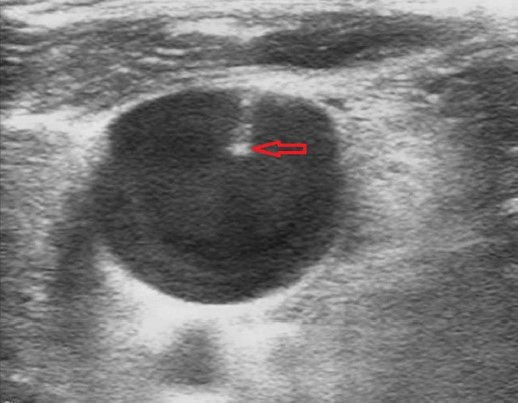
\includegraphics[width=0.5\textwidth]{igla}
\centering
\caption{Wizualizacja ig�y wk�uwanej do �y�y szyjnej wewn�trznej w badaniu USG (przekr�j poprzeczny). Czerwon� strza�k� oznaczono ko�c�wk� ig�y \cite{spacekUseUltrasoundGuidance2018a}.}\label{igla}
\end{figure}

USG uk�adu krwiono�nego mo�e by� r�wnie� wykorzystywane nie tylko w celach diagnostycznych, ale r�wnie� do planowania zabieg�w chirurgicznych takich jak endarterektomia t�tnic szyjnych CEA (ang. \textit{Carotid Endarterectomy}). Jest to uznana metoda leczenia mia�d�ycy t�tnicy szyjnej i polega ona na operacyjnym usuni�ciu, a dok�adnie wyci�ciu blaszek mia�d�ycowych ze �wiat�a naczynia. Powstaj�ca wewn�trz t�tnicy blaszka mia�d�ycowa skutkuje zw�eniem, a nawet zamkni�cie jej �wiat�a. Mia�d�yca t�tnic szyjnych jest powa�n� przyczyn� wyst�pienia udaru niedokrwiennego m�zgu. W zwi�zku z tym endarterektomia na wczesnych etapach mia�d�ycy staje si� skuteczn� form� leczenia. Aby przeprowadzi� taki zabieg istotna jest bardzo dok�adna lokalizacja blaszek ze wzgl�du na ich niewielkie wymiary oraz mo�liwo�� uszkodzenia wra�liwej struktury jak� jest t�tnica. Dzi�ki USG przedoperacyjnemu mo�na dostatecznie okre�li� miejsca wyst�puj�cych zmian i odpowiednio zaplanowa� proces operacji. Wspomagaj�cym rozwi�zaniem staj� si� systemy dokonuj�ce segmentacji naczy� wraz z blaszkami mia�d�ycowymi. Dzi�ki temu mo�na okre�li� ich wielko�� (np. d�ugo��, obj�to�� w przypadku rekonstrukcji 3D) oraz pole przekroju ograniczonego �wiat�a t�tnicy w danym miejscu, a nast�pnie po przeprowadzonej endarterektomii dokona� analizy por�wnawczej z uzyskanymi rezultatami \cite{norrisUltrasoundSufficientVascular2004, hassanRobustSpatialFuzzy2019a, chengCarotidPlaqueSegmentation2018a}. 


Analiz� stanu naczy� krwiono�nych wykonuje si� r�wnie� stosuj�c r�ne modalno�ci standardowego USG. Przyk�adem mo�e by� USG Doopler, polegaj�ce na obserwowaniu przep�ywu krwi. Ultrasonografia Dopplerowska wykorzystuje rozproszenie fali d�wi�kowej na poruszaj�cym si� obiekcie (np. przep�ywaj�cych w naczyniach krwinkach), dzi�ki czemu pozwala na zdobycie informacji o pr�dko�ci z jak� przemieszcza si� obserwowany obiekt. Na tej podstawie mo�na dokona� oceny, w kt�rych miejscach przep�yw krwi jest wolniejszy oraz gdzie przep�yw jest zablokowany. W jednym z rodzaj�w badania z wykorzystaniem zjawiska Dopplera obserwowa� mo�na kolorystyk� poruszaj�cych si� szybko obiekt�w odpowiedni� w zale�no�ci od kierunku przep�ywu. Elementy statyczne pozostaj� w odcieniach szaro�ci.
W wyniku analizy t�tnic i �y� przy u�yciu tej techniki, mo�na obliczy� maksymaln� warto�� pr�dko�ci lub obj�to�� krwi przep�ywaj�c� przez naczynie przypadaj�c� na jednostk� czasu \cite{troianosGuidelinesPerformingUltrasound2011a, spacekUseUltrasoundGuidance2018a, worldhealthorganizationIMAIDistrictClinician2012}. 

Inn� odmian� klasycznego USG jest wewn�trznaczyniowe obrazowanie ultrad�wi�kami IVUS (ang. \textit{Intravascular Ultrasound}). Technika ta polega na wytworzeniu obraz�w przekroj�w poprzecznych podczas prowadzenia cewnika wewn�trz naczy� krwiono�nych. Dzi�ki temu mo�na zaobserwowa� �wiat�o naczy� jak i struktur� �ciany naczyniowej. W ostatnich latach technologia ta sta�a si� bardzo przydatna w analizie choroby mia�d�ycowej. Zapewnia informacja o charakterze zmiany mia�d�ycowej oraz kszta�cie i wielko�� blaszki mia�d�ycowej. Zbadano r�wnie� inne zastosowanie IVUS jakim sta�a si� implantacja stent�w. Automatyczne rozwi�zania do segmentacji �cian naczy� oraz analizy blaszek mia�d�ycowych pozwalaj� na uzyskanie wi�kszej dok�adno�ci oraz podejmowania szybszych dzia�a� w obliczu diagnozy i leczenia pacjent�w \cite{cardinalIntravascularUltrasoundImage2006a}.


\subsection{Standard DICOM}\label{dic}
Rozw�j sprz�tu przeznaczonego do obrazowania medycznego, wdra�anych do u�ytku przez r�nych producent�w, wymusi� opracowanie standardu przechowywania i wymiany obraz�w medycznych. Dzi�ki wprowadzeniu wzorca DICOM (ang. \textit{Digital Imaging and Communication in Medicine}). Wymiana obraz�w medycznych sta�a si� �atwiejsza, szybsza i bezpieczniejsza pomi�dzy systemami informatycznych (np. RIS (ang. Radiology Information System), PACS (ang. Picture Archiving and Communication System)). Aktualna wersja (3.0) zosta�a opublikowana przez NEMA (ang. \textit{National Electrical Manufacturers Association}) w 1993 roku. Opr�cz podstawowych danych obrazowych format takiego pliku (.dicom) przechowuje przydatne metadane takie jak: dane pacjenta, dane jednostki wykonuj�cej badanie, dat�, rodzaj badania, informacje dotycz�ce cech obrazu oraz wiele innych. Standard DICOM posiada wa�n� zalet�-- umo�liwia dalsz� rozbudow� i aktualizacj� stale rozwijaj�cych si� modu��w. Z puntu widzenia szybkiego post�pu w dziedzinie obrazowania jest to bardzo przydatna cecha \cite{mildenbergerIntroductionDICOMStandard2002, mustraOverviewDICOMStandard2008}.





\subsection{Analiza obrazowa wspomagana komputerowo}\label{diag}
Post�p technologiczny aparatury przeznaczonej do obrazowania medycznego zapewnia coraz lepsz� jako�� uzyskiwanych obraz�w. Dzi�ki wysokiej rozdzielczo�ci mo�liwe staje si� projektowanie automatycznych system�w przeznaczonych do analizy medycznej, niejednokrotnie przewy�szaj�cych mo�liwo�ci ekspert�w. Takie rozwi�zania mo�na podzieli� na klasyczne oraz te z u�yciem sztucznej inteligencji. 

Przetwarzanie obraz�w jest szerokim poj�ciem, obejmuj�cym wiele r�nych metod maj�cych na celu analiz� lub/oraz modyfikacj� cech obrazowych w celu poprawy jego parametr�w lub poszukiwania okre�lonych wzorc�w. Przyk�adem mo�e by� wykrywanie tekstur, kszta�t�w, czy kontur�w. W tym obszarze zastosowanie nierzadko znajduj� filtry (cz�sto stosowane do og�lnej poprawy jako�ci), maj�ce na celu wyeksponowanie danych struktur w obrazie np. kraw�dzi (filtr Canny'ego, Laplace'a). Przydatne s� r�wnie� operacje morfologiczne, dzi�ki kt�rym mo�liwa jest modyfikacja cech geometrycznych obiekt�w. Bardzo warto�ciowym na wielu polach zabiegiem jest proces segmentacji. Polega on na podziale obrazu na regiony (zbiory pikseli) podobne wzgl�dem siebie wed�ug pewnych przyj�tych w�asno�ci np. poziomy szaro�ci. Istnieje wiele metod klasycznych wykorzystywanych do segmentacji poszukiwanych obiekt�w w obrazie. S� nimi: progowanie (np. Otsu), rozrost i/lub podzia� obszaru, dopasowanie wzorca lub metody kraw�dziowe np. aktywny kontur (ang. \textit{active contour}). Innym obszarem z zakresu przetwarzania obrazowego jest klasyfikacja na przyk�ad poprzez grupowanie lub z u�yciem metod statystycznych \cite{doughertyDigitalImageProcessing2020}. 


Zupe�nie inaczej do analizy obrazowej odnosi si� poj�cie sztucznej inteligencji. Termin AI jest stosowany, chc�c zdefiniowa� proces na�ladowania funkcji poznawczych takich jak uczenie si� i rozwi�zywanie problem�w. Innymi s�owy sztuczna inteligencja to systemy, realizuj�ce zadania, kt�re zwykle wymagaj� ludzkiej inteligencji. W obszarze AI mo�emy wyr�ni� poj�cie uczenia maszynowego ML (ang. \textit{Machine Learning}), kt�re oznacza uczenie si� na podstawie dostarczonych danych bez wyra�nego zaprogramowania. Przyk�adami takich rozwi�za� s�: analiza g��wnych sk�adowych PCA (ang. principal component analysis), maszyna wektor�w no�nych SVM (support vector machines) oraz sztuczne sieci neuronowe ANN (ang. artificial neural networks). Architektura sieci neuronowej sk�ada si� z warstw, z�o�onych z po��czonych ze sob� neuron�w. Ka�dy neuron wykonuje wa�on� sum� danych wej�ciowych, kt�re s�
nast�pnie przekazywane do funkcji aktywacji. Wagi s� dobierane dynamicznie na etapie treningu. Mo�na wyr�ni� nast�puj�ce typy warstw: warstwa wej�ciowa (przyjmuje dane wej�ciowe), warstwa wyj�ciowa (dostarcza wyniki przetwarzania danych) i warstwa ukryta (wyodr�bnia cechy analizowanych danych). Najnowsze osi�gni�cia dotycz� podzbioru ML, jakim jest g��bokie uczenie DL (ang. Deep Learning). S� to metody uczenia oparte na sieciach neuronowych, kt�re dokonuj� samodzielnego uczenia, poprzez rozpoznawanie wzorc�w z zastosowaniem wielu warstw przetwarzania. Spo�r�d r�nych rozwi�za� g��bokiego uczenia splotowe sieci neuronowe CNN (ang. Convolution Neural Network) mo�na uzna� za wysoko cenione i wykorzystywane w wielu dziedzinach �ycia ludzkiego. CNN s� niezwykle cennym narz�dziem w zakresie analizy obrazowej, szczeg�lnie w zakresie medycznym 
\cite{tangRoleArtificialIntelligence2020,kimDeepLearningBiomedical2020,pesapaneArtificialIntelligenceMedical2018}. 


\section{Rozwi�zania alternatywne}
Ze wzgl�du na specyfik� tematu pracy i brak dost�pnych rozwi�za� realizuj�cych w ca�o�ci temat niniejszej pracy przegl�d alternatywnych metod podzielono na dwa obszary--- segmentacja naczy� krwiono�nych w obrazach ultrasonograficznych oraz pomiar naczynia krwiono�nego na podstawie wcze�niej uzyskanej maski. Dodatkowym argumentem przemawiaj�cym za takim podzia�em pracy jest mo�liwo�� wykorzystywania obraz�w segmentacyjnych do r�nych zastosowa�. Maski struktur czy obiekt�w anatomicznych s� warto�ciowymi danymi, pozwalaj�cymi na dalsz� i g��bsz� analiz� w konkretnym obszarze. 
\subsection{Segmentacja naczy� krwiono�nych w obrazach USG}\label{wielkosc}
Problem segmentacji danych obiekt�w na obrazie mo�na podzieli� na dwie podstawowe grupy: metody klasyczne oraz metody opieraj�ce si� na  uczeniu maszynowym. Przyk�adem rozwi�za� pierwszego typu jest u�ycie transformaty Hough'a (ang. \textit{Hough Transform}), kt�ra wykrywa regularne kszta�ty np. okr�gi (kszta�t naczy� w widoku przekrojowym obrazu ultrasonograficznego jest najbardziej zbli�ony do okr�gu). Opiera si� na wyznaczeniu prawdopodobie�stwa wyst�pienia danego obiektu w ka�dym punkcie obrazu. Takie podej�cie zaproponowali: Spyretta Golemati, John Stoitsis, Emmanouil G. Sifakis, Thomas Balkizas oraz Konstantina S. Nikita w pracy zatytu�owanej,,\textit{Using the hough transform to segment ultrasound images of longitudinal and transverse sections of the carotid artery}'' \cite{golematiUsingHoughTransform2007}. Inn� technik� wykorzystali autorzy pracy o tytule ,,\textit{Ultrasound Common Carotid Artery Segmentation Based on Active Shape Model}'' \cite{yangUltrasoundCommonCarotid2013}, w kt�rej to opisali wykrywanie granic �ciany naczynia krwiono�nego z zastosowaniem modeli aktywnych kszta�t�w (ang. \textit{Active Shape Models}). Metoda polega na statystycznym dopasowaniu kszta�tu wej�ciowego do obiektu zainteresowania poprzez iteracyjne odkszta�canie. Ciekawe rozwi�zanie przedstawili Amr R. Abdel-Dayem i Mahmoud R. El-Sakka w pracy ,,\textit{Carotid Artery Ultrasound Image Segmentation Using Fuzzy Region Growing}'' \cite{abdel-dayemCarotidArteryUltrasound2005}, gdzie na podstawie punktu startowego przeprowadzony jest algorytm wzrostu rozmytego regionu (ang. \textit{Fuzzy Region Growing}). Jego wynikiem jest rozmyta mapa po��cze�, kt�ra zostaje poddana progowaniu. \\
\indent Istnieje wiele innych klasycznych technik, pozwalaj�cych wykry� kontur i uzyska� mask� segmentowanego naczynia. 
Mimo niezbyt skomplikowanej implementacji takich algorytm�w s� one nierzadko p�automatyczne, co oznacza, �e konieczna jest ingerencja u�ytkownika, najcz�ciej na pocz�tkowym etapie procesu (np. poprzez wyb�r punktu pocz�tkowego, nale��cego do obiektu). W zwi�zku z tym wyniki s� mocno zale�ne od dok�adno�ci dzia�a� cz�owieka. Kolejn� wad� tego typu strategii jest znaczny wp�yw jako�ci obrazu (np. obecno�� szumu, artefakt�w, kontrast), kt�r� nie zawsze da si� skorygowa� w wystarczaj�cym stopniu, na dzia�anie algorytmu. Upraszczaj�c, mo�na stwierdzi�, �e maj�c do czynienia z gorszym jako�ciowo obrazem nale�y liczy� si� z mniej dok�adnym wynikiem.  Niekt�re z tych metod s� kosztowne obliczeniowo i tym samym czasoch�onne. Bior�c pod uwag� powy�sze argumenty oraz kwesti� ci�g�ego rozwoju i bada� nad rewolucyjnymi, w pe�ni automatycznymi i szeroko stosowanymi metodami z zakresu uczenia maszynowego, postanowiono dokona� przegl�du alternatywnych dzia�a� w�a�nie w tym zakresie. \\
\indent 
W pracy ,,\textit{Automatic localization of Common Carotid Artery in ultrasound images using Deep Learning}'' \cite{hassaninAutomaticLocalizationCommon2021} zaproponowano podej�cie wykrywania t�tnicy szyjnej CCA (ang. \textit{Common Carotid Artery}) w obrazach ultrasonograficznych z wykorzystaniem szybkiej rekurencyjnej splotowej sieci neuronowej (ang. \textit{Faster R-CNN}), aby wykry� prostok�tny region zainteresowania (ang. \textit{Object bounding box}), zawieraj�cy CCA. Nast�pnie przeprowadzono kilka r�nych technik lokalizacyjnych (np. aktywny kontur), aby dok�adnie wyznaczy� granic� t�tnicy. Wsp�czynnik Jaccarda'a, w odniesieniu do obraz�w prawdy (ang. \textit{ground truth}), wyni�s� oko�o 0,91. Na takich wynikach w �atwy spos�b mo�na uzyska� maski analizowanych obiekt�w. 

Inne podej�cie przestawia artyku� ,,\textit{Deep learning methods for detection of carotid artery wall}'' \cite{anic2021deep}, w kt�rym to autorzy podejmuj� zadanie segmentacji CCA przy pomocy sieci CNN SegNet i por�wnuj� wyniki ze zmodyfikowan� g��bok� sieci� konwolucyjn� oparta na modelu U-Net. Zaproponowane rozwi�zanie (CNN SegNet) osi�gn�o nieco lepszy wynik, plasuj�cy si� na poziomie 0,92 wg. wska�nika Dice'a. 

W kolejnej z pracy o tytule ,,\textit{Two-stage and dual-decoder convolutional U-Net ensembles for reliable vessel and plaque segmentation in carotid ultrasound images}'' \cite{xieTwostageDualdecoderConvolutional2020a} wykorzystano zmodyfikowany model sieci U-Net do przygotowania dw�ch metod--- dwuetapowego kaskadowego po��czenia U-Net oraz podw�jnego dekodera U-Net. Pierwsza z nich osi�gn�a wska�nik Dice'a wynosz�cy 0,95, natomiast druga 0,91. 



Publikacja pt. ,,\textit{Segmentation of common and internal carotid arteries from 3D ultrasound images based on adaptive triple loss}'' \cite{jiangSegmentationCommonInternal2021a} prezentuje metod� segmentacji CCA za pomoc� dwukana�owej sieci U-Net. Zastosowano podej�cie z trzykrotn� segmentacj� na podstawie wej�ciowych obraz�w ich odwr�conych wersji. Ostateczna maska segmentacji zosta�a wygenerowana poprzez tzw. g�osowanie wi�kszo�ciowe. Uzyskane przez autor�w wyniki w postaci wska�nika Dice'a wynosz� 95\%.

Leah A. Groves, Blake VanBerlo, Natan Veinberg, Abdulrahman Alboog, Terry M. Peters oraz Elvis C. S. Chen w swojej pracy ,,\textit{Automatic segmentation of the carotid artery and internal jugular vein from 2D ultrasound images for 3D vascular reconstruction}'' \cite{grovesAutomaticSegmentationCarotid2020b} por�wnuj� sie� Mask R-CNN oraz U-Net oparte na algorytmach automatycznego segmentowania t�tnicy szyjnej i �y�y szyjnej wewn�trznej w obrazach ultrasonograficznych. Do szkolenia obydwu modeli zastosowano czterokrotn� walidacj� krzy�ow�. Algorytm U-Net zawiera� dodatkowo etap przetwarzania ko�cowego, w kt�ry ostateczn� segmentacje stanowi� najwi�kszy po��czony obszar dla ka�dej klasy (CCA oraz IJV). Mask R-CNN jest z kolei rozbudowan� wersj� szybkiej rekurencyjnej splotowej sieci neuronowej (Faster R-CNN), jednak opr�cz dostarczenia dw�ch wyj�ciowych danych tj. \textit{Object bounding box} oraz klasy obiektu, sie� przekazuje r�wnie� wynik segmentacji tego obiektu. Zawiera ona kilka sieci sk�adowych w tym m.in. ResNet-50. �rednie wyniki segmentacji dla CCA i IJV, na podstawie wska�nika Dice'a uzyskane przez mask� R-CNN wynios�y 0,90 i 0,88 odpowiednio. Zmodyfikowana ko�cowo sie� U-Net osi�gn�a wynik na poziomie 0,81 oraz 0,71 dla CCA i IJV.


\subsection{Pomiar naczynia krwiono�nego}\label{wielkosc}


Ka�de z przytoczonych rozwi�za� skutkuje r�nymi rezultatami, a odpowiedni wyb�r powinien by� dostosowany do danego problemu. 




\section{Cel pracy}
Celem pracy jest stworzenie automatycznego systemu maj�cego za zadanie okre�lenie wielko�ci naczy� krwiono�nych w obrazach ultrasonograficznych. Wymaga to realizacji nast�puj�cych etap�w:
\begin{itemize}
 \item zebranie danych-- rejestracja obraz�w ultrasonograficznych naczy� krwiono�nych oraz przegl�d otwarto-�r�d�owych baz obraz�w,
 \item przegl�d dost�pnych rozwi�za� i wyb�r narz�dzi,
 \item opracowanie algorytmu segmentacji naczy� krwiono�nych z obraz�w USG,
 \item opracowanie metody pomiaru wielko�ci naczynia krwiono�nego na podstawie segmentacji,
 \item testowanie systemu.
\end{itemize}



\section{Uk�ad pracy}

\chapter{Metodologia}\label{Chapter_Metodologia}



\chapter{Cz�� konstrukcyjna/Specyfikacja wewn�trzna}


\chapter{Instrukcja obs�ugi/Specyfikacja zewn�trzna}

\chapter{Rezultaty}


\chapter{Podsumowanie}



\appendix  % <--- zaczynaj� si� dodatki; jak nazywa si� rozdzia� -> szuka� appendixname powy�ej
%\chapter{Dodatek A}
W dodatku umieszczamy opis ewentualnych znanych algorytm�w, z kt�rych korzystamy proponuj�c w�asn� metodologi�, opisan� w rozdziale~\ref{Chapter_Metodologia}. Wykaz pozycji literaturowych tworzymy w oddzielnym pliku \texttt{Praca.bib}. Chc�c si� odwo�a� w tek�cie do wybranej pozycji bibliograficznej korzystamy z komendy \texttt{cite}. Efekt jej u�ycia dla kilku pozycji jednocze�nie to~\cite{Tadeusiewicz,Malina,Nieniewski_Morfologia}.

%%%%%%%%%%%%%%%%%%%%%%%%%%%%%%%%%%%%%%%%%%%%%%%%%%%%%%%%%%%%%%%%%%%%%%%%%%%%%%%%%%%%%%%%%%%%%%%%%%%%%%%%%%%%%%%%%%%%%%%%%%%%%%%%%%%%%%%%%%%%%%%%%%%%%%%%%%%%%%%%%%%%%%%
\chapter{Dodatek B}
Podstawowe kwestie techniczne dotycz�ce wzor�w, rysunk�w, tabel poni�ej.

Wzory tworzymy w �rodowisku \texttt{equation}. Chc�c odwo�a� si� do wybranego wzoru gdzie� w tek�cie nale�y nada� mu stosown�, niepowtarzaln� i jednoznaczn� etykiet�, po ty by m�c np. napisa� zdanie: ze wzoru~\ref{Wzor_Dodawanie} wynika \ldots
\begin{equation}\label{Wzor_Dodawanie}
	c = a + b
\end{equation}

Wzory z�o�one, charakteryzuj�ce si� przypisaniem warto�ci zmiennej w pewnych okoliczno�ciach tworzymy przy u�yciu otoczenia \texttt{eqnarray}. Odwo�anie do wzoru jak wcze�niej. 
\begin{eqnarray}\label{equ_progowanie}
    BW & = & \left \{
    \begin{array}{ll}
      1, & I(x,y) \geq T \\
      0, & I(x,y) < T\\
    \end{array}
    \right.,
\end{eqnarray}

% \subsection{Usuwanie numeracji przy r�wnaniach}

Numeracj� r�wna� mo�na tymczasowo (w~danej linijce) wy��czy� poprzez u�ycie $\backslash{}nonumber$
\begin{eqnarray}
	a_i = a_{i-1}+a_{i-2}\nonumber \\ % w tej linijce nie ma numeru
              +a_{i-3}
\end{eqnarray}


\section{Wstawianie rysunk�w}
Rysunki umieszczamy w otoczeniu \texttt{figure}, centruj�c je w poziomie komend� \texttt{centering}. Rozmiary rysunku ustalamy w komendzie \texttt{includegraphics} dobieraj�c wielko�� wzgl�dem rozmiaru strony lub bezwzgl�dnie np. w cm. Ponadto najpierw zapowiadamy pojawienie si� rysunku w tek�cie (czyli np. Na rysunku (Rys~\ref{Rysunek_LogoIB}) pracy, a dopiero p�niej wstawiamy sam rysunek. Dodatkowo sterowa� mo�emy umiejscowieniem rysunku na stronie dzi�ki parametrom \texttt{[!htb]} okre�laj�cym miejsce. Odpowiednio s� to: \texttt{here}, \texttt{top}, \texttt{bottom}. 
\begin{figure}[!htb]
	\centering
	
\includegraphics[width=.35\textwidth]{logoRIB}
	\caption{Logo Wydzia�u In�ynierii Biomedycznej.}\label{Rysunek_LogoIB}
\end{figure}

Do��czaj�c rysunki nie trzeba podawa� rozszerzenia (wr�cz jest to odradzane). Je�li rysunki znajduj� si� w~katalogu \emph{rysunki}, nie trzeba r�wnie� podawa� �cie�ki do nich.

\section{Wstawianie tabelek}
Analogicznie post�pujemy z tabelkami, z t� r�nic� �e tworzymy j� w otoczeniu \texttt{table}. W nim natomiast sam� tabel� definiujemy albo w �rodowisku \texttt{tabular}, albo \texttt{tabularx}. Podobnie z odwo�aniami w tek�cie: najpierw odwo�anie w Tab.~\ref{Tabelka_Tabela}, a dopiero p�niej sama tabela.
\begin{table}[!htb]
	\centering
	\topcaption{Opis nad tabelk�.}\label{Tabelka_Tabela}
	\begin{tabular}{|c|c|c|c|} \hline \hline 
		Kolumna 1 & Kolumna 2 & Kolumna 3 & Kolumna 4 \\ \hline
		Wiersz 1 & & & \\ \hline
		Wiersz 2 & & & \\ \hline
		Wiersz 3 & & & \\ \hline
		& & & \\ \hline
		& & & \\ \hline
	\end{tabular}
\end{table}

%%%%%%%%%%%%%%%%%%%%%%%%%%%%%%%%%%%%%%%%%%%%%%%%%%%%%%%%%%%%%%%%%%%%%%%%%%%%%%%%%%%%%%%%%%%%%%%%%%%%%%%%%%%%%%%%%%%%%%%%%%%%%%%%%%%%%%%%%%%%%%%%%%%%%%%%%%%%%%%%%%%%%%%
\chapter{Kwestie edytorskie}
Zbi�r zasad pomocnych przy redagowaniu tekstu pracy wystarczaj�co szczeg�owo przedstawia ksi��ka~\cite{Chwalowski}.

Uwaga! Pisz�c prac� nale�y zwr�ci� uwag� na nast�puj�ce kwestie:
\begin{enumerate}
	\item Prace piszemy w formie bezosobowej.
	\item Unikamy okre�le� potocznych, spolszcze� funkcjonuj�cych codziennej mowie itp.
	\item Pos�uguj�c si� znanymi nam (a nie czytelnikowi) has�ami (r�wnie� skr�tami, akronimami) najpierw je definiujemy i~t�umaczymy, a~dopiero p�niej traktujemy za znane.
	\item Podpisy pod rysunkami lub nad tabelami traktujemy jak zdania, a wi�c powinny stanowi� sp�jn� ca�o�� oraz powinny zosta� zako�czone kropk�.
	\item Podobnie wypunktowania (po dwukropku kolejne punkty pisane ma�ymi literami, oddzielane przecinkami, ostatni zako�czony kropk� o ile ko�czy zdanie).
	\item Do ka�dego rysunku, tabeli, pozycji bibliograficznej musi istnie� odwo�anie w tek�cie pracy, przy czym do pierwszych dw�ch musi si� ono pojawi� zanim umie�cimy rysunek/tabel�.
\end{enumerate}


\clearpage \addcontentsline{toc}{chapter}{\bibname}
\bibliography{MGRdolatexa}


\end{document}
